% Propósito: organizar las medidas de control según el eslabón físico sobre el
% que actúan y separar transmisión, reflexión y protección.
% Origen: sección \ref{sec:u10-control}; esquema cualitativo sin prestaciones.
% Descripción accesible: una cadena conecta fuente, trayecto y receptor. Debajo
% de la fuente aparecen reducción de generación y encapsulado; debajo del
% trayecto se separan transmisión y reflexiones; debajo del receptor aparecen
% distancia, tiempo, organización y protección. Las tres familias de acciones
% apuntan a un bloque común: el resultado se evalúa como cambio de una métrica
% entre condiciones declaradas.
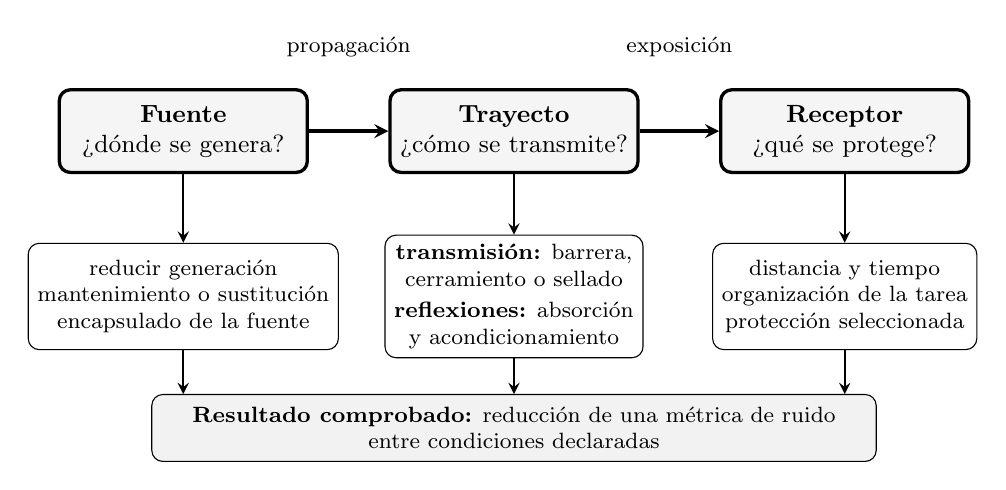
\begin{tikzpicture}[
    x=1cm,
    y=1cm,
    >=stealth,
    font=\small,
    etapa/.style={
        draw,
        rounded corners,
        very thick,
        minimum width=3.15cm,
        minimum height=1.05cm,
        align=center,
        fill=black!4
    },
    accion/.style={
        draw,
        rounded corners,
        minimum width=3.15cm,
        minimum height=1.35cm,
        align=center,
        font=\footnotesize
    },
    resultado/.style={
        draw,
        rounded corners,
        minimum width=9.20cm,
        minimum height=0.85cm,
        align=center,
        fill=black!5,
        font=\footnotesize
    }
]
    \node[etapa] (fuente) at (1.90,4.25)
        {\textbf{Fuente}\\¿dónde se genera?};
    \node[etapa] (trayecto) at (6.10,4.25)
        {\textbf{Trayecto}\\¿cómo se transmite?};
    \node[etapa] (receptor) at (10.30,4.25)
        {\textbf{Receptor}\\¿qué se protege?};

    \draw[->,very thick] (fuente) -- (trayecto)
        node[midway,above=23pt,font=\footnotesize] {propagación};
    \draw[->,very thick] (trayecto) -- (receptor)
        node[midway,above=23pt,font=\footnotesize] {exposición};

    \node[accion] (accion-f) at (1.90,2.15)
        {reducir generación\\
         mantenimiento o sustitución\\
         encapsulado de la fuente};
    \node[accion] (accion-t) at (6.10,2.15)
        {\textbf{transmisión:} barrera,\\
         cerramiento o sellado\\[2pt]
         \textbf{reflexiones:} absorción\\
         y acondicionamiento};
    \node[accion] (accion-r) at (10.30,2.15)
        {distancia y tiempo\\
         organización de la tarea\\
         protección seleccionada};

    \draw[->,thick] (fuente) -- (accion-f);
    \draw[->,thick] (trayecto) -- (accion-t);
    \draw[->,thick] (receptor) -- (accion-r);

    \node[resultado] (resultado) at (6.10,0.48)
        {\textbf{Resultado comprobado:} reducción de una métrica de ruido\\
         entre condiciones declaradas};
    \draw[->,thick] (accion-f.south) -- (1.90,0.91);
    \draw[->,thick] (accion-t.south) -- (6.10,0.91);
    \draw[->,thick] (accion-r.south) -- (10.30,0.91);
\end{tikzpicture}
